% Relatorio do T2 - Filas de Prioridade (Estrutura de Dados A, UFSM 2026/2)
% Formatacao ABNT (NBR 14724, NBR 6023, NBR 10520) seguindo o MDT da UFSM
% Compilar: latexmk -pdf relatorio.tex
\documentclass[12pt,openany,oneside,a4paper,english,brazil,sumario=tradicional]{abntex2}

\usepackage[T1]{fontenc}
\usepackage[utf8]{inputenc}
\usepackage{lmodern}
\usepackage{mathptmx}
\usepackage{graphicx}
\usepackage{fancyvrb}
\usepackage{array}

% ---------- secoes no padrao do MDT/UFSM ----------
% primaria: MAIUSCULAS e negrito; secundaria: MAIUSCULAS sem negrito
\renewcommand{\ABNTEXchapterfont}{\rmfamily\bfseries}
\renewcommand{\ABNTEXchapterfontsize}{\normalsize}
\renewcommand{\ABNTEXsectionfont}{\rmfamily\mdseries}
\renewcommand{\ABNTEXsectionfontsize}{\normalsize}
\renewcommand{\ABNTEXsubsectionfont}{\rmfamily\bfseries}
\renewcommand{\ABNTEXsubsectionfontsize}{\normalsize}

\setlength{\parindent}{1.25cm}
\setlength{\parskip}{0pt}

% quadros (informacao textual), numerados em sequencia no documento todo
\newcommand{\quadroname}{Quadro}
\newfloat{quadro}{loq}{\quadroname}

% legendas em fonte reduzida, separadas por travessao
\captionnamefont{\ABNTEXfontereduzida}
\captiontitlefont{\ABNTEXfontereduzida}
\captiondelim{ -- }

% pseudocodigos e saidas em quadro fechado, espacamento simples
\fvset{fontsize=\small, frame=single, framesep=3mm, baselinestretch=1}

% ---------- dados do trabalho ----------
\titulo{FILAS DE PRIORIDADE: HEAPS BINÁRIOS E IMPLEMENTAÇÃO EM C}
\autor{Diego Kelme Santos da Silva\\Gabriel Sangoi\\Pedro Klein}
\local{Santa Maria, RS}
\data{2026}
\orientador[Professora:]{Deise de Brum Saccol}
\instituicao{}
\tipotrabalho{Relatório}
\addto\captionsbrazil{\renewcommand{\contentsname}{SUMÁRIO}}
\preambulo{Relatório apresentado à disciplina de Estrutura de Dados A, do Curso de Graduação em Sistemas de Informação da Universidade Federal de Santa Maria (UFSM, RS), como requisito parcial para avaliação do Trabalho T2.}

\makeatletter
\hypersetup{
  pdftitle={Filas de prioridade: heaps binários e implementação em C},
  pdfauthor={Diego Kelme Santos da Silva, Gabriel Sangoi, Pedro Klein},
  pdfsubject={Estrutura de Dados A - Trabalho T2},
  colorlinks=true, linkcolor=black, citecolor=black, filecolor=black, urlcolor=black,
  bookmarksdepth=4
}
\makeatother

% capa no modelo do MDT/UFSM
\renewcommand{\imprimircapa}{%
  \begin{capa}%
    \centering
    {\bfseries UNIVERSIDADE FEDERAL DE SANTA MARIA\\
    CENTRO DE TECNOLOGIA\\
    CURSO DE GRADUAÇÃO EM SISTEMAS DE INFORMAÇÃO\par}
    \vspace*{4cm}
    {\imprimirautor\par}
    \vfill
    {\bfseries\imprimirtitulo\par}
    \vfill
    \vspace*{3cm}
    \imprimirlocal\\
    \imprimirdata
  \end{capa}
}

\begin{document}

\selectlanguage{brazil}
\frenchspacing

% ================= PRE-TEXTUAIS =================
\pretextual
\imprimircapa
\imprimirfolhaderosto*

\pdfbookmark[0]{\contentsname}{toc}
\tableofcontents*
\cleardoublepage

% ================= TEXTUAIS =================
\textual
\pagestyle{simple}
\aliaspagestyle{chapter}{simple}

\chapter{INTRODUÇÃO}

As estruturas de dados são essenciais na criação de programas, pois possibilitam a organização, o armazenamento e a manipulação de informações de forma eficiente. Conforme a aplicação, várias estruturas podem ser empregadas para satisfazer as exigências de organização e acesso às informações. Entre elas, sobressaem as filas de prioridade, que possibilitam ordenar elementos conforme sua relevância ou prioridade.

Ao contrário de uma fila convencional, onde os elementos são normalmente processados na sequência em que são adicionados, uma fila de prioridade leva em conta o valor de prioridade relacionado a cada item. Assim, um item com prioridade superior pode ser processado antes de outros que foram adicionados antes.

Uma das maneiras mais eficazes de implementar filas de prioridade é através dos heaps binários (CORMEN \emph{et al.}, 2022; SEDGEWICK; WAYNE, 2011). Essa estrutura emprega uma árvore binária completa e adota regras específicas de disposição dos elementos, possibilitando operações como inserção e remoção com custo logarítmico.

Os heaps binários podem ser divididos em duas categorias principais: heap máximo e heap mínimo. No primeiro, o maior elemento fica na raiz da árvore, enquanto, no segundo, o menor elemento assume essa posição. Essa propriedade possibilita acessar de forma rápida o elemento com a maior ou a menor prioridade, conforme o tipo empregado.

O propósito deste trabalho é expor os conceitos essenciais dos heaps binários, explicar suas características e ilustrar o funcionamento das operações principais executadas nessa estrutura. Será apresentada também uma implementação na linguagem C, centrada em um heap máximo armazenado em vetor, possibilitando ver na prática como os elementos são adicionados, retirados e rearranjados para manter as propriedades da estrutura.

\chapter{DEFINIÇÃO DE HEAP BINÁRIO}

Um heap binário é uma estrutura de dados disposta como uma árvore binária completa, que respeita uma determinada propriedade de ordenação entre os seus nós (CORMEN \emph{et al.}, 2022). Essa estrutura é amplamente empregada na criação de filas de prioridade, pois possibilita manter os elementos organizados sem necessitar de uma ordenação total após cada operação.

Para entender seu funcionamento, é essencial conhecer duas características principais: a estrutura da árvore e a propriedade do heap.

A primeira característica é que o heap deve ser uma árvore binária completa. Isso implica que todos os níveis da árvore precisam estar totalmente preenchidos, exceto, possivelmente, o último nível. Os elementos desse nível final devem ser organizados da esquerda para a direita, sem que haja espaços vazios entre as posições.

A segunda característica diz respeito à comparação dos valores entre os nós. Conforme o tipo de heap empregado, o valor de cada pai precisa ser maior ou igual (ou menor ou igual) aos valores de seus filhos. Essa regra deve ser seguida em toda a estrutura para que ela continue sendo um heap válido.

Há duas categorias principais de heap binário, que se distinguem pela regra de comparação entre os elementos: o heap máximo e o heap mínimo.

\section{HEAP MÁXIMO}

O heap máximo é uma estrutura de dados onde o valor de cada nó pai deve ser sempre maior ou igual ao valor de seus filhos. Essa regra vale em todos os níveis da árvore, assegurando que nenhum filho tenha um valor maior que o de seu pai. A Figura~\ref{fig:max} mostra um exemplo.

\begin{figure}[htb]
  \caption{\label{fig:max}Exemplo de heap de máximo}
  \centering
  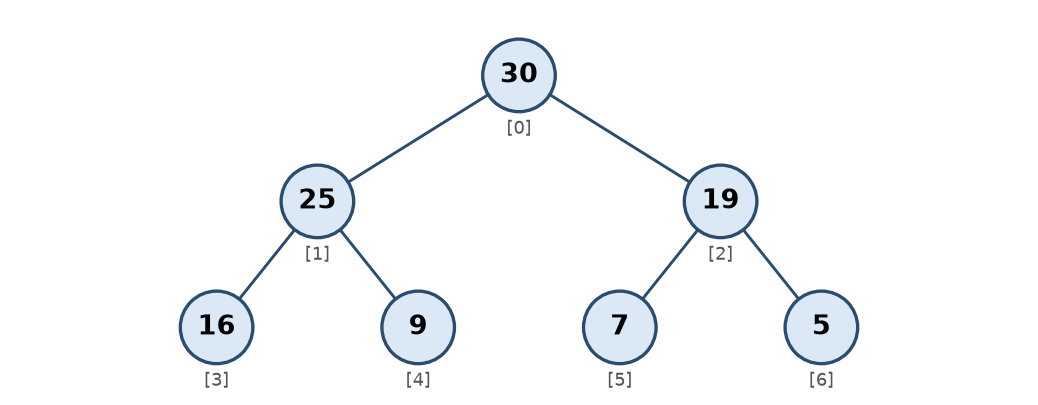
\includegraphics[width=0.62\textwidth]{figuras/fig_heap_maximo.png}
  \fonte{Elaborado pelos autores (2026).}
\end{figure}

Devido a essa característica, o maior elemento da estrutura estará sempre posicionado na raiz da árvore. Isso possibilita que o programa obtenha diretamente o maior valor guardado, sem a necessidade de examinar todos os elementos.

Uma característica fundamental do heap máximo é que seus elementos não precisam estar totalmente ordenados. A estrutura apenas requer que cada pai seja maior ou igual aos seus filhos, não havendo a necessidade de que os valores estejam em ordem decrescente ao se percorrer os níveis da árvore. Na Figura~\ref{fig:max}, por exemplo, o 16 está em um nível mais baixo que o 19, mas é menor que ele apenas por coincidência: os dois estão em ramos diferentes e não são comparados.

Essa estrutura torna o heap máximo particularmente valioso na criação de filas de prioridade, onde é essencial identificar rapidamente os elementos de maior prioridade. Como o valor máximo permanece sempre na raiz, sua consulta pode ser feita em tempo constante, ou seja, com complexidade $O(1)$.

Contudo, sempre que um elemento é adicionado ou retirado, pode ser preciso reestruturar a árvore para manter essa característica. Para isso, são empregados os procedimentos Upheap e Downheap, que movimentam os elementos entre os níveis da árvore. No desenvolvimento deste trabalho foi empregado exatamente o heap máximo: a implementação em C mantém o valor máximo na raiz e faz uso de comparações e trocas para manter a ordem da estrutura.

\section{HEAP MÍNIMO}

O heap mínimo possui uma estrutura parecida com a do heap máximo, mas aplica a regra oposta: o valor de cada nó pai deve ser sempre menor ou igual aos valores dos seus filhos. A Figura~\ref{fig:min} mostra um heap mínimo com os mesmos valores da Figura~\ref{fig:max}.

\begin{figure}[htb]
  \caption{\label{fig:min}Exemplo de heap de mínimo}
  \centering
  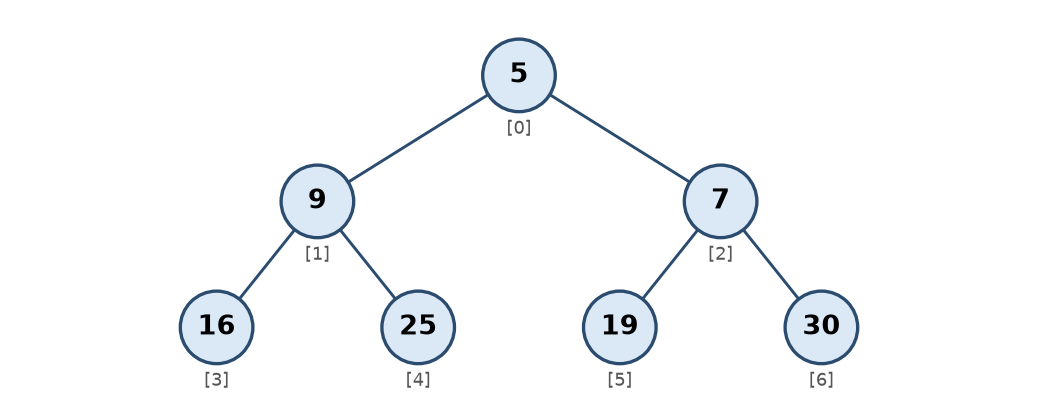
\includegraphics[width=0.62\textwidth]{figuras/fig_heap_minimo.png}
  \fonte{Elaborado pelos autores (2026).}
\end{figure}

Essa característica assegura que o menor elemento existente na estrutura permaneça sempre na raiz da árvore. Dessa forma, quando há a necessidade de obter o menor valor guardado, não é preciso passar por todos os elementos, pois ele pode ser achado diretamente na posição inicial do heap.

Assim como no heap máximo, os elementos de um heap mínimo não precisam estar totalmente ordenados. A estrutura assegura apenas que cada pai tenha um valor menor ou igual aos valores de seus descendentes, mantendo essa regra em todos os níveis da árvore.

O heap mínimo é empregado em circunstâncias em que é necessário localizar rapidamente o item de menor valor ou prioridade. Um exemplo de uso é o algoritmo de Dijkstra, empregado para descobrir caminhos mínimos em grafos, no qual uma fila de prioridade ajuda na escolha do próximo vértice a ser analisado (CORMEN \emph{et al.}, 2022).

O heap máximo e o heap mínimo compartilham a mesma estrutura de árvore binária completa e aplicam processos semelhantes para a inserção e a reorganização. A diferença principal está na condição aplicada para comparar os elementos. Assim, enquanto o heap máximo coloca o maior elemento na raiz, o heap mínimo coloca o menor elemento nesse lugar. A escolha entre os dois varia conforme a necessidade da aplicação.

\chapter{PROPRIEDADES DOS HEAPS BINÁRIOS}

Os heaps binários têm características particulares que asseguram sua estrutura e possibilitam que suas operações sejam executadas de forma eficiente. Essas características estão ligadas tanto ao formato da árvore quanto à maneira como os elementos são dispostos nela.

A primeira característica é a de árvore binária completa: todos os níveis da árvore precisam estar totalmente preenchidos, exceto, possivelmente, o último, que é preenchido da esquerda para a direita, sem deixar espaços entre os elementos.

A segunda característica diz respeito à disposição dos valores. No heap máximo, cada nó pai deve ter um valor maior ou igual aos valores de seus filhos. No heap mínimo, cada nó pai deve ter um valor menor ou igual ao dos seus filhos. Essa regra deve ser seguida em todos os níveis da estrutura.

Outra característica significativa é que um heap não representa uma árvore completamente ordenada. A estrutura assegura somente a relação entre cada nó e seus filhos, não criando uma ordem total entre todos os elementos. Assim, não é necessário que os valores estejam dispostos em ordem crescente ou decrescente ao percorrer a árvore ou o vetor.

Além disso, a altura de um heap binário com $n$ elementos é $\lfloor \log_2 n \rfloor$ (CORMEN \emph{et al.}, 2022). Isso ocorre porque a estrutura é uma árvore completa, em que cada nível comporta o dobro de nós do nível anterior. Essa propriedade impacta diretamente a eficiência das operações de inserção e de reorganização, que percorrem no máximo um caminho da raiz até uma folha.

Por último, é fundamental ressaltar que essas características devem ser mantidas após qualquer operação que altere a estrutura. Por essa razão, os heaps empregam procedimentos específicos, como Upheap e Downheap, que são responsáveis por reestruturar os elementos quando necessário.

\chapter{REPRESENTAÇÃO DE UM HEAP BINÁRIO EM VETOR}

Uma das grandes vantagens dos heaps binários é a capacidade de guardar seus elementos diretamente em um vetor, eliminando a necessidade de usar ponteiros para ligar os diversos nós da árvore.

Essa representação é viável graças à característica de árvore binária completa. Já que os elementos são dispostos da esquerda para a direita em cada nível, suas localizações seguem uma ordem previsível dentro do vetor: a raiz ocupa a posição 0, seus filhos ocupam as posições 1 e 2, os filhos destes ocupam as posições 3 a 6, e assim por diante.

Levando em conta que os índices iniciam em zero, é possível determinar diretamente a localização do pai e dos filhos de qualquer elemento (MORIN, 2013). Para isso, são empregadas as seguintes fórmulas, em que $i$ é o índice do elemento examinado:

\begin{itemize}
  \item posição do pai: $(i - 1) / 2$;
  \item posição do filho esquerdo: $2i + 1$;
  \item posição do filho direito: $2i + 2$.
\end{itemize}

Uma vez que os índices são números inteiros, a divisão usada para determinar o pai considera apenas a parte inteira do resultado. A Figura~\ref{fig:vetor} mostra o heap da Figura~\ref{fig:max} armazenado em vetor e aplica as fórmulas ao índice 1.

\begin{figure}[htb]
  \caption{\label{fig:vetor}Heap de máximo armazenado em vetor, com índices a partir de 0}
  \centering
  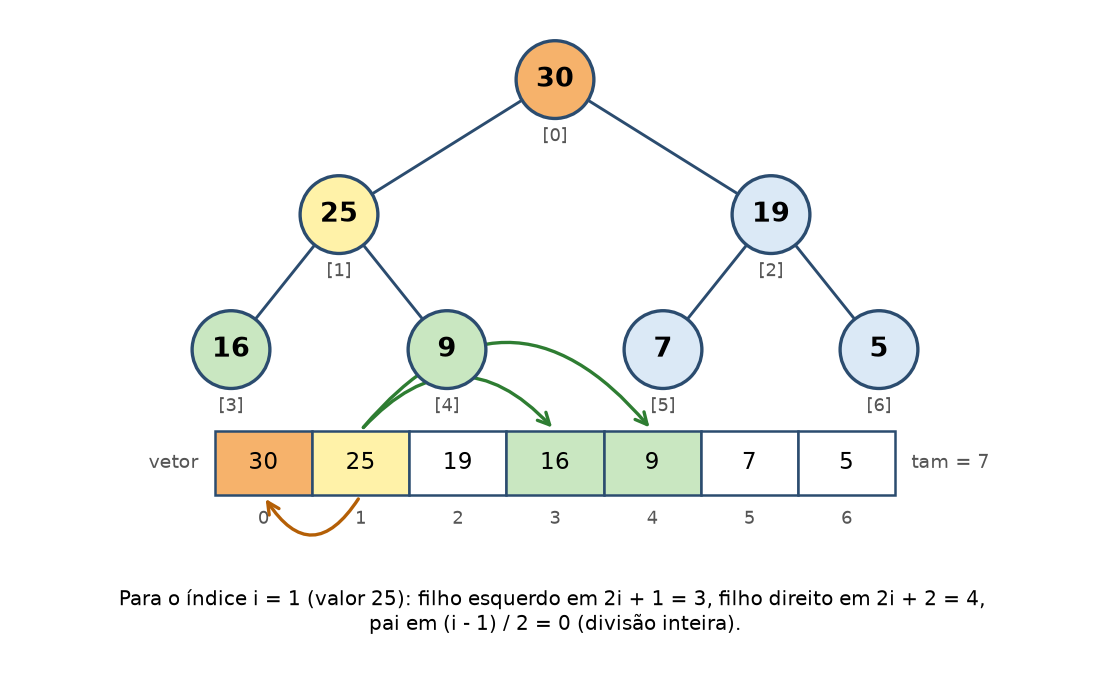
\includegraphics[width=0.78\textwidth]{figuras/fig_vetor_indices.png}
  \fonte{Elaborado pelos autores (2026).}
\end{figure}

O uso dessas fórmulas torna a navegação pela estrutura mais simples, pois possibilita encontrar os elementos conectados sem a necessidade de explorar toda a árvore. Além disso, elimina a necessidade de guardar referências ou endereços de memória para cada nó.

Na implementação deste trabalho, o heap é representado por um vetor de inteiros, com a capacidade máxima definida pela constante \texttt{MAX}, cujo valor é 150. A estrutura possui uma variável denominada \texttt{tam}, que indica quantos elementos estão armazenados atualmente. Essa variável é fundamental, pois possibilita reconhecer quais posições do vetor estão preenchidas, gerenciar as inserções e evitar que sejam incluídos elementos além da capacidade disponível.

Assim, o armazenamento em vetor facilita a implementação, tornando-a mais organizada e possibilitando a utilização de operações aritméticas simples para acessar os elementos da árvore.

\chapter{OPERAÇÕES PRINCIPAIS DE UM HEAP BINÁRIO}

As operações principais executadas em um heap binário são a inserção, a remoção e a reestruturação dos elementos. Essas operações asseguram que a estrutura preserve suas características essenciais, garantindo que o elemento de maior ou menor prioridade fique na posição correta, conforme o tipo de heap empregado.

No heap máximo, empregado na implementação deste trabalho, o maior elemento deve sempre estar na raiz da árvore. Para assegurar essa característica após mudanças na estrutura, são empregados processos de reorganização denominados Upheap e Downheap, também conhecidos como ajuste para cima e ajuste para baixo (SEDGEWICK; WAYNE, 2011).

\section{INSERÇÃO DE ELEMENTOS}

A inserção envolve acrescentar um novo elemento ao heap sem prejudicar suas características. Para isso, o elemento é primeiramente colocado na próxima posição disponível da estrutura, ou seja, logo após o último elemento do vetor que representa a árvore.

Essa posição é importante porque mantém a propriedade de árvore binária completa. Contudo, apenas adicionar o elemento não assegura que a propriedade de ordenação do heap continue a ser mantida. Em um heap máximo, por exemplo, o valor novo pode ser maior que o seu pai, exigindo que a organização da estrutura seja refeita.

Depois de adicionar o elemento, o procedimento Upheap é acionado. Ele compara o novo valor com os seus ancestrais e efetua as trocas necessárias até que a propriedade do heap seja restaurada.

A inserção tem complexidade $O(\log n)$, pois, no cenário mais desfavorável, o elemento pode atravessar toda a altura da árvore até chegar à raiz. Como a altura de um heap binário completo cresce de maneira logarítmica em relação ao número de elementos, a quantidade de operações requeridas também é proporcional a $\log n$.

\section{PROCEDIMENTO UPHEAP}

O procedimento Upheap, também chamado de subida ou ajuste ascendente, é utilizado principalmente após a adição de um novo elemento. Seu objetivo é assegurar que a propriedade de ordem do heap máximo seja preservada.

O processo inicia na posição onde o novo item foi colocado. Calcula-se o índice do pai e comparam-se os dois valores. Se o elemento atual for maior que seu pai, os valores são trocados de lugar. Esse procedimento se repete enquanto o elemento permanecer maior que seu pai e termina quando o elemento atinge a raiz ou quando encontra um pai com valor maior ou igual ao seu.

A Figura~\ref{fig:insercao} mostra, passo a passo, a inserção do valor 45 em um heap máximo com cinco elementos. O 45 entra no índice 5 e sobe duas vezes até chegar à raiz. Visualizações interativas do mesmo processo estão disponíveis no OpenDSA (VIRGINIA TECH, [20--]).

\begin{figure}[p]
  \caption{\label{fig:insercao}Passo a passo da inserção do valor 45 (Upheap)}
  \centering
  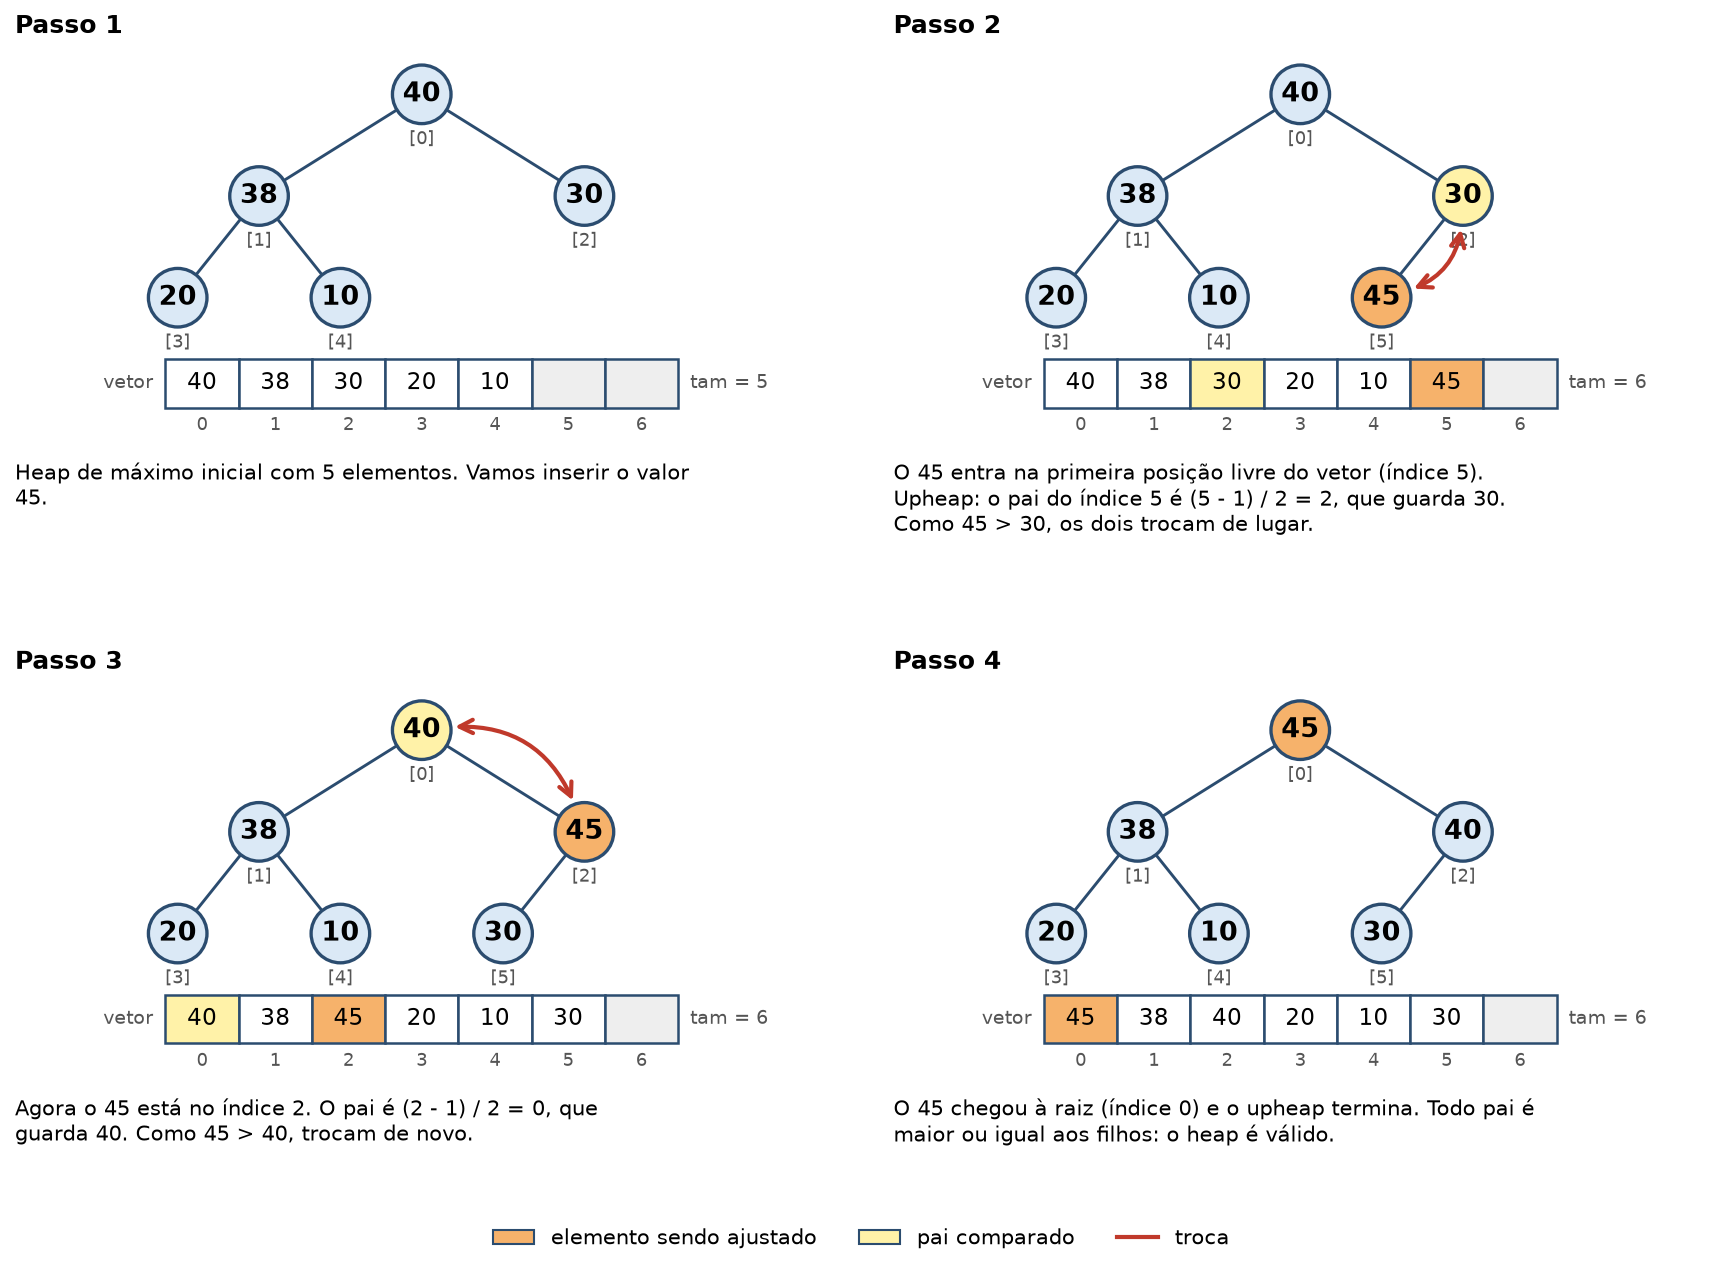
\includegraphics[width=\textwidth]{figuras/fig_insercao_upheap.png}
  \fonte{Elaborado pelos autores (2026).}
\end{figure}

No heap máximo, esse processo assegura que nenhum filho tenha um valor maior que o de seu pai. Assim, a estrutura continua seguindo a propriedade de ordem definida.

Na implementação em C deste trabalho, a função \texttt{upHeap} executa esse procedimento utilizando a fórmula do índice do pai, $(i - 1) / 2$. A função sobe pelos níveis da árvore conforme necessário, executando as trocas até que a posição correta do elemento seja encontrada.

A complexidade do processo é $O(\log n)$, já que o elemento pode subir, no máximo, a altura da árvore.

\section{REMOÇÃO DE ELEMENTOS}

A remoção é uma operação central em uma fila de prioridade. Na sua forma clássica, em um heap máximo, o item retirado é o que está na raiz, porque representa o maior valor e, portanto, detém a maior prioridade (SEDGEWICK; WAYNE, 2011).

Para executar essa remoção, o valor da raiz é substituído pelo último elemento presente no heap. Em seguida, o tamanho da estrutura é diminuído, desconsiderando a posição que anteriormente abrigava o último elemento. Como o novo valor da raiz pode não seguir a propriedade de ordem, é preciso realizar o procedimento Downheap para reestruturar a árvore. Na implementação deste trabalho, essa é a opção 2 do menu, executada pela função \texttt{removeMaior}.

Além da remoção clássica, a implementação também permite remover um valor específico informado pelo usuário (opção 4 do menu). Para isso, o programa utiliza a função \texttt{buscaNo}, que percorre o vetor e encontra a posição onde o valor informado está guardado. Após localizar o elemento, sua posição recebe o último elemento do heap, e o tamanho da estrutura é reduzido.

Depois dessa troca, a estrutura da árvore deve ser recuperada. Conforme o valor que passou a ocupar a posição, pode ser necessário fazer um ajuste para cima ou para baixo. Assim, a estrutura mantém a propriedade de heap máximo.

É relevante enfatizar que a remoção de um valor específico inclui uma fase extra em relação à remoção da raiz: a procura pelo elemento. Uma vez que essa busca percorre o vetor, sua complexidade é $O(n)$. O ajuste posterior tem complexidade $O(\log n)$, mas o custo total da operação permanece $O(n)$, em razão da busca.

\section{PROCEDIMENTO DOWNHEAP}

O procedimento Downheap, também chamado de descida ou ajuste para baixo, é aplicado quando um elemento deve ser movido para os níveis inferiores da árvore para que a propriedade de ordem do heap seja recuperada.

No heap máximo, o processo compara o elemento em questão com seus filhos à esquerda e à direita. Se algum dos filhos tiver um valor maior, é preciso fazer uma troca. Quando há dois filhos, deve-se escolher aquele que possui o maior valor, já que ele ficará acima do outro filho e a propriedade do heap precisa se manter.

Após a troca, o processo continua a partir da nova posição do elemento. Esse procedimento se repete até que o elemento esteja em uma posição onde seja maior ou igual aos seus filhos, ou até atingir uma posição sem filhos.

A Figura~\ref{fig:remocao} mostra, passo a passo, a remoção da raiz do heap obtido na Figura~\ref{fig:insercao}. O último elemento (30) vai para a raiz e desce uma vez, trocando de lugar com o maior filho (40).

\begin{figure}[p]
  \caption{\label{fig:remocao}Passo a passo da remoção da raiz (Downheap)}
  \centering
  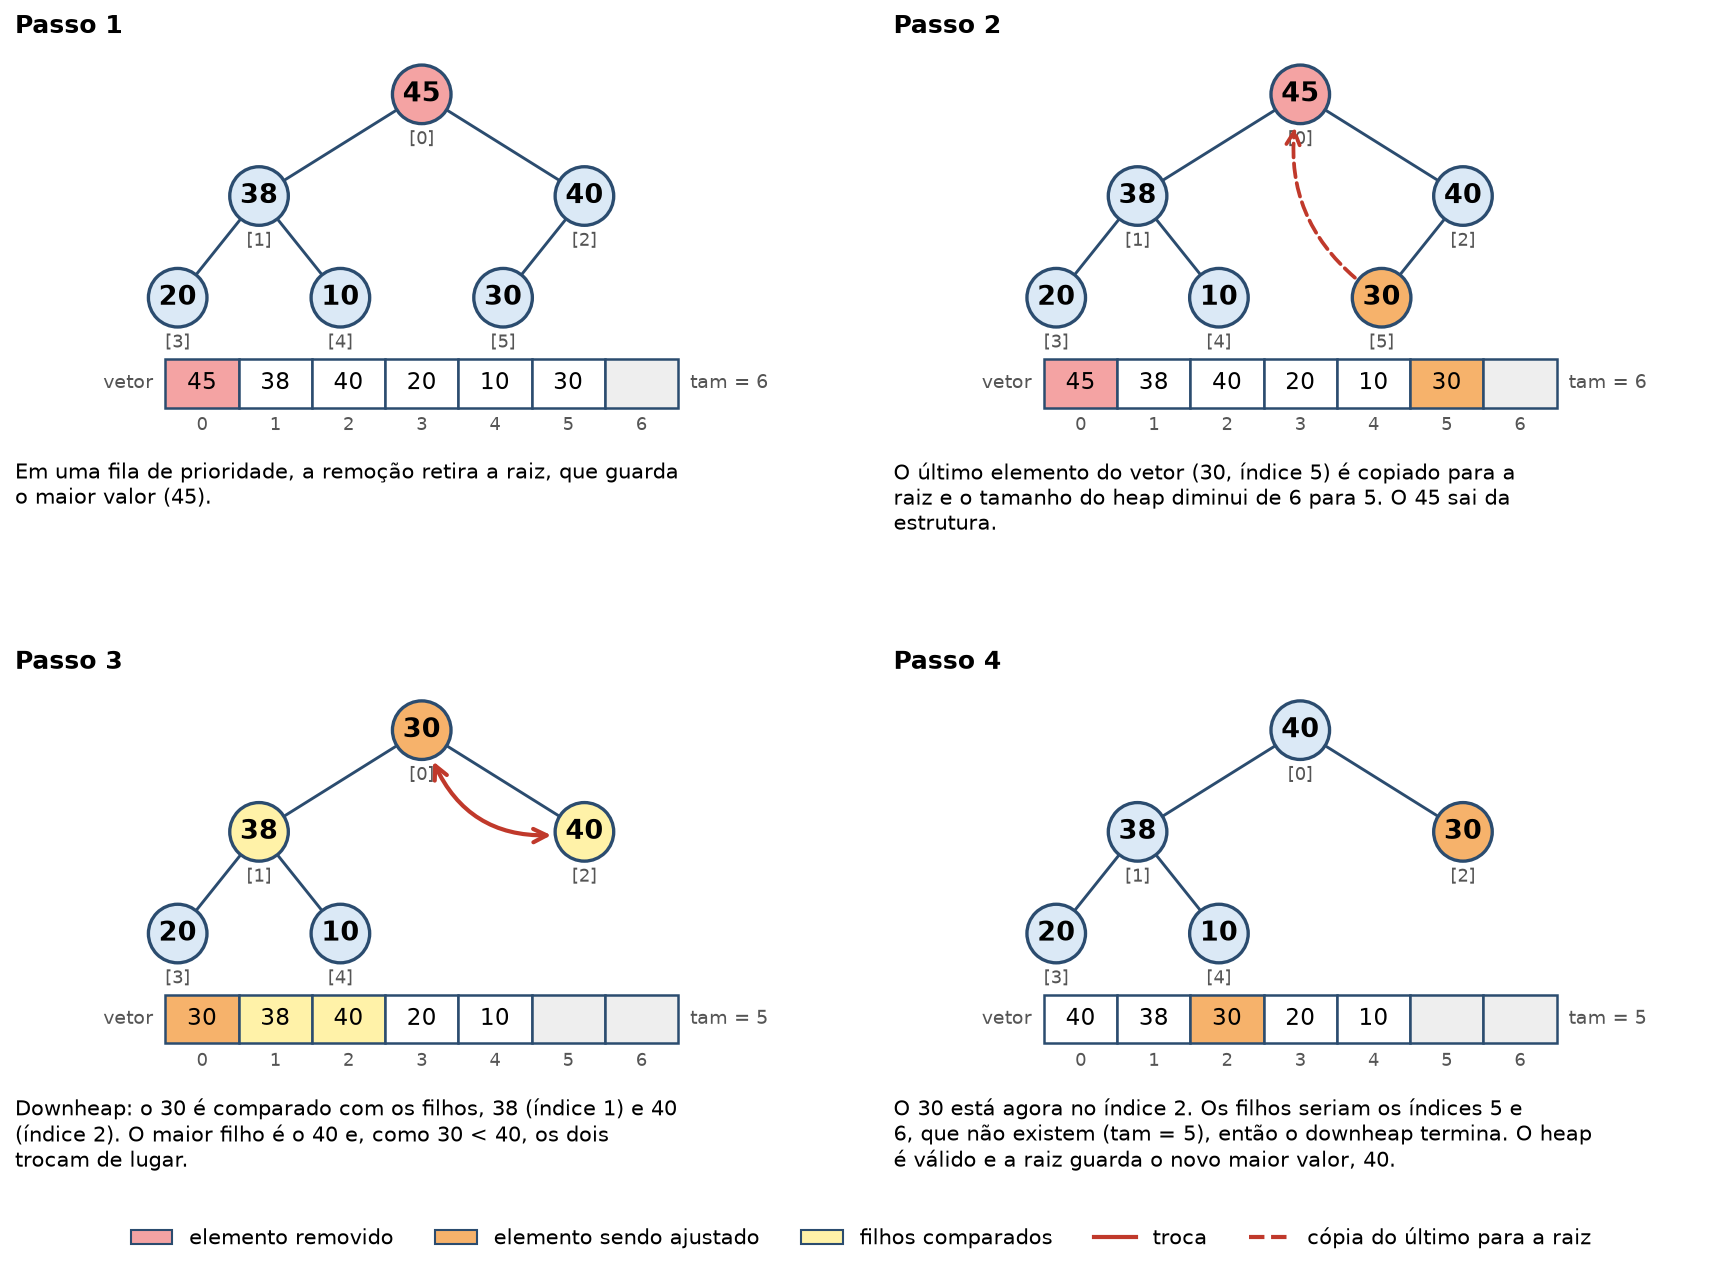
\includegraphics[width=\textwidth]{figuras/fig_remocao_downheap.png}
  \fonte{Elaborado pelos autores (2026).}
\end{figure}

Na implementação em C, a função \texttt{downHeap} executa essas comparações utilizando os índices dos filhos esquerdo e direito. O processo verifica quais posições existem dentro do tamanho atual do heap, identifica o maior filho e efetua a troca quando necessário.

Assim como o Upheap, o Downheap também apresenta complexidade $O(\log n)$, já que, no pior cenário, o elemento pode atravessar todos os níveis da árvore até alcançar a posição final.

\chapter{ALGORITMOS EM PSEUDOLINGUAGEM}

Os pseudocódigos representam a lógica das operações de forma simplificada, independentemente de uma linguagem de programação específica. Eles ajudam na compreensão dos processos empregados e mostram a ordem das etapas essenciais para operar um heap binário.

Dado que a implementação deste trabalho utiliza um heap máximo, os pseudocódigos a seguir assumem que o maior elemento deve estar na raiz e que cada pai deve ter um valor maior ou igual ao de seus filhos. Em todos eles, \texttt{tam} é a quantidade atual de elementos e \texttt{pai(i)} vale $(i - 1) / 2$.

\section{INSERÇÃO}

O procedimento de inserção adiciona um novo elemento na próxima posição disponível do heap e, depois disso, chama o procedimento Upheap para restabelecer a propriedade de ordem (Quadro~\ref{qua:inserir}).

\begin{quadro}[htb]
\caption{\label{qua:inserir}Pseudocódigo da inserção}
\begin{Verbatim}
INSERIR(heap, valor)
    SE heap estiver cheio
        RETORNAR

    heap[tam] = valor
    tam = tam + 1

    UPHEAP(heap, tam - 1)
FIM
\end{Verbatim}
\fonte{Elaborado pelos autores (2026).}
\end{quadro}

Inicialmente, o algoritmo verifica se existe espaço disponível para armazenar um novo elemento. Caso exista, o valor é colocado na primeira posição livre do vetor e o tamanho do heap é atualizado. Em seguida, o procedimento Upheap é executado para garantir que o novo elemento esteja na posição adequada.

\section{UPHEAP}

O procedimento Upheap compara o elemento com seu pai, realizando trocas enquanto o elemento atual possuir valor maior (Quadro~\ref{qua:upheap}).

\begin{quadro}[htb]
\caption{\label{qua:upheap}Pseudocódigo do Upheap}
\begin{Verbatim}
UPHEAP(heap, i)
    ENQUANTO i > 0
        p = (i - 1) / 2

        SE heap[i] > heap[p]
            TROCAR heap[i] com heap[p]
            i = p
        SENÃO
            PARAR
    FIM ENQUANTO
FIM
\end{Verbatim}
\fonte{Elaborado pelos autores (2026).}
\end{quadro}

O algoritmo começa na posição do elemento que precisa ser ajustado. Enquanto ele não estiver na raiz, calcula o índice de seu pai e compara os valores. Se o elemento atual for maior, ocorre uma troca e o processo continua na posição do pai. Caso contrário, a execução termina, pois a propriedade de ordem já está sendo respeitada.

\section{REMOÇÃO DO MAIOR ELEMENTO}

A remoção clássica de uma fila de prioridade retira a raiz. O último elemento ocupa o lugar dela e o procedimento Downheap restaura a propriedade de ordem (Quadro~\ref{qua:removermaior}).

\begin{quadro}[htb]
\caption{\label{qua:removermaior}Pseudocódigo da remoção do maior elemento}
\begin{Verbatim}
REMOVER_MAIOR(heap)
    SE tam == 0
        INFORMAR que o heap está vazio
        RETORNAR

    maior = heap[0]
    heap[0] = heap[tam - 1]
    tam = tam - 1

    DOWNHEAP(heap, 0)
    RETORNAR maior
FIM
\end{Verbatim}
\fonte{Elaborado pelos autores (2026).}
\end{quadro}

\section{DOWNHEAP}

O procedimento Downheap ajusta um elemento em direção aos níveis inferiores da árvore. Ele compara o elemento com seus filhos e realiza trocas quando algum deles apresenta valor maior (Quadro~\ref{qua:downheap}).

\begin{quadro}[htb]
\caption{\label{qua:downheap}Pseudocódigo do Downheap}
\begin{Verbatim}
DOWNHEAP(heap, i)
    ENQUANTO verdadeiro
        esq = 2 * i + 1
        dir = 2 * i + 2
        maior = i

        SE esq < tam E heap[esq] > heap[maior]
            maior = esq

        SE dir < tam E heap[dir] > heap[maior]
            maior = dir

        SE maior == i
            PARAR

        TROCAR heap[i] com heap[maior]
        i = maior
    FIM ENQUANTO
FIM
\end{Verbatim}
\fonte{Elaborado pelos autores (2026).}
\end{quadro}

O algoritmo calcula os índices dos filhos esquerdo e direito e verifica quais deles existem dentro do tamanho atual do heap. Em seguida, identifica o maior valor entre o elemento atual e seus filhos. Caso o maior valor continue sendo o do próprio elemento, a propriedade de ordem está preservada e o procedimento termina. Caso contrário, ocorre uma troca com o maior filho, e o processo continua a partir da nova posição do elemento.

\section{REMOÇÃO DE UM VALOR ESPECÍFICO}

Além da remoção da raiz, a implementação deste trabalho permite que o usuário indique qual valor pretende retirar do heap. Por essa razão, antes de efetuar a troca, é preciso encontrar a posição do elemento desejado (Quadro~\ref{qua:removervalor}).

\begin{quadro}[htb]
\caption{\label{qua:removervalor}Pseudocódigo da remoção de um valor específico}
\begin{Verbatim}
REMOVER(heap, valor)
    i = BUSCAR(heap, valor)
    SE i não existir
        INFORMAR que o valor não foi encontrado
        RETORNAR

    heap[i] = heap[tam - 1]
    tam = tam - 1

    SE i < tam
        SE i > 0 E heap[i] > heap[pai(i)]
            UPHEAP(heap, i)
        SENÃO
            DOWNHEAP(heap, i)
    FIM SE
FIM
\end{Verbatim}
\fonte{Elaborado pelos autores (2026).}
\end{quadro}

Inicialmente, o algoritmo busca o valor fornecido pelo usuário. Se ele não for localizado, a operação termina sem alterar o heap. Ao localizar o elemento, sua posição recebe o valor que estava na última posição do vetor e o tamanho da estrutura é diminuído. Por último, verifica-se se o elemento que ocupou a posição deve subir ou descer na árvore: se ele for maior que seu pai, executa-se o Upheap; do contrário, o ajuste é feito pelo Downheap.

\chapter{ANÁLISE DE COMPLEXIDADE}

A análise de complexidade possibilita entender a eficiência das operações executadas em uma estrutura de dados. Em se tratando de heaps binários, a maior parte das operações de rearranjo tem complexidade logarítmica, uma vez que a altura da árvore é proporcional a $\log n$ (CORMEN \emph{et al.}, 2022).

Essa propriedade torna os heaps eficazes em situações que requerem, com frequência, a inserção de elementos e a consulta ou remoção dos valores de maior prioridade. O Quadro~\ref{qua:complexidade} resume as complexidades das operações empregadas neste trabalho.

\begin{quadro}[htb]
\caption{\label{qua:complexidade}Complexidade das operações do heap}
\centering
\small
\begin{tabular}{|p{4.2cm}|>{\centering\arraybackslash}p{2.6cm}|p{7cm}|}
\hline
\textbf{Operação} & \textbf{Complexidade} & \textbf{Justificativa} \\ \hline
Acesso à raiz & $O(1)$ & A raiz está sempre na primeira posição do vetor. \\ \hline
Inserção & $O(\log n)$ & O novo elemento pode precisar subir pela altura da árvore. \\ \hline
Upheap & $O(\log n)$ & O elemento pode percorrer os níveis em direção à raiz. \\ \hline
Downheap & $O(\log n)$ & O elemento pode percorrer os níveis em direção às folhas. \\ \hline
Remoção da raiz & $O(\log n)$ & A substituição é seguida por um ajuste para baixo. \\ \hline
Busca por valor & $O(n)$ & No pior caso, é necessário percorrer todo o vetor. \\ \hline
Remoção de valor específico & $O(n)$ & A busca linear domina o custo da operação, seguida pelo ajuste logarítmico. \\ \hline
Impressão do heap & $O(n)$ & Todos os elementos são percorridos para exibição. \\ \hline
\end{tabular}
\fonte{Elaborado pelos autores (2026).}
\end{quadro}

A complexidade da remoção varia conforme a maneira como ela é executada. Quando a meta é remover a raiz, não é preciso localizar o elemento, uma vez que sua posição é conhecida. Por esse motivo, essa operação possui complexidade $O(\log n)$.

Na opção 4 do programa, por outro lado, o usuário escolhe um valor específico para remover. Como o heap não ordena os elementos de forma completa, não se pode saber de antemão em que posição esse valor está. Assim, a função de busca deve percorrer os elementos até localizar o valor desejado, o que resulta em complexidade $O(n)$.

Portanto, mesmo que o heap binário possibilite procedimentos eficientes de inserção e reorganização, a localização de um elemento qualquer ainda é linear. Essa propriedade deve ser levada em conta ao optar por essa estrutura em diferentes aplicações.

\chapter{IMPLEMENTAÇÃO EM LINGUAGEM C}

A implementação desenvolvida neste trabalho utiliza a linguagem C para representar e manipular um heap máximo por meio de um vetor. O programa permite inserir elementos, remover o maior elemento, remover um valor específico, visualizar a estrutura e encerrar a execução por meio de um menu interativo. O código está no arquivo \texttt{heap.c}, entregue junto com este relatório.

Para organizar o código, foram utilizadas funções específicas para cada operação. Essa divisão facilita a compreensão da implementação, evita a repetição desnecessária de instruções e permite que cada procedimento seja responsável por uma tarefa bem definida.

\section{ESTRUTURA DE DADOS}

A representação do heap foi realizada através de uma \texttt{struct}, que inclui um vetor de inteiros e uma variável que armazena a quantidade atual de elementos (Quadro~\ref{qua:struct}).

\begin{quadro}[htb]
\caption{\label{qua:struct}Estrutura que representa o heap}
\begin{Verbatim}
#define MAX 150

typedef struct heap {
    int heap[MAX];
    int tam;
} Heap;
\end{Verbatim}
\fonte{Elaborado pelos autores (2026).}
\end{quadro}

O vetor tem capacidade máxima de 150 posições, determinada pela constante \texttt{MAX}. A variável \texttt{tam} mostra quantos elementos estão realmente guardados na estrutura. Essa representação possibilita empregar o vetor para simular uma árvore binária completa, sem a exigência de criar estruturas individuais para cada nó ou usar ponteiros para interligar os elementos. Como os índices iniciam em zero, as posições dos pais e dos filhos são determinadas pelas fórmulas apresentadas no Capítulo~4.

\section{FUNÇÕES IMPLEMENTADAS}

O programa foi dividido em funções, cada uma responsável por uma operação específica do heap:

\begin{itemize}
  \item \texttt{criaHeap}: inicializa a estrutura, definindo o tamanho inicial como zero;
  \item \texttt{pai}, \texttt{esquerda} e \texttt{direita}: calculam, respectivamente, o índice do pai, do filho esquerdo e do filho direito de um nó;
  \item \texttt{troca}: troca de posição um elemento do vetor com o seu pai; é usada durante os procedimentos de reorganização do heap;
  \item \texttt{insere}: lê valores informados pelo usuário até que ele digite \texttt{s}; cada valor é colocado na próxima posição disponível e ajustado com \texttt{upHeap};
  \item \texttt{upHeap}: ajusta um elemento em direção à raiz, comparando-o com seu pai e efetuando as trocas necessárias para manter a propriedade de heap máximo;
  \item \texttt{removeMaior}: remove a raiz (o maior valor), informa qual valor foi removido, coloca o último elemento na raiz e chama \texttt{downHeap};
  \item \texttt{buscaNo}: procura um valor específico no vetor e retorna sua posição, ou $-1$ quando ele não existe;
  \item \texttt{removeHeap}: remove um valor escolhido pelo usuário, usando \texttt{buscaNo}; a posição encontrada recebe o último elemento do heap, o tamanho é reduzido e o elemento é ajustado com \texttt{upHeap} e \texttt{downHeap};
  \item \texttt{downHeap}: ajusta um elemento em direção aos níveis inferiores da árvore, trocando-o com o maior filho enquanto ele for menor que esse filho;
  \item \texttt{imprime}: percorre o vetor e mostra, para cada nó, o seu valor e os valores dos filhos esquerdo e direito; quando um filho não existe, mostra \texttt{vazio};
  \item \texttt{menu}, \texttt{leInt} e \texttt{leStr}: mostram o menu e fazem a leitura das entradas, rejeitando valores que não são números inteiros.
\end{itemize}

\section{FUNCIONAMENTO DO PROGRAMA}

A interação com o usuário ocorre por meio de um menu apresentado no terminal, que permite selecionar qual operação deverá ser executada sem precisar modificar o código-fonte. As opções disponibilizadas são:

\begin{itemize}
  \item 1 -- inserir um ou mais elementos;
  \item 2 -- remover o maior elemento (a raiz);
  \item 3 -- imprimir o heap;
  \item 4 -- remover um valor específico;
  \item 0 -- sair do programa.
\end{itemize}

Quando o usuário escolhe a opção de inserção, o programa solicita valores em sequência, até que seja digitado \texttt{s}, e cada valor é inserido com o ajuste necessário para preservar a propriedade de heap máximo. Na opção 2, o programa retira a raiz, informa o valor removido e reorganiza a estrutura. Na opção 4, o usuário informa o valor que deseja retirar; o programa procura esse elemento e, caso ele seja encontrado, realiza a substituição e a reorganização da estrutura.

A opção de impressão mostra cada nó do heap, na ordem em que aparece no vetor, com o seu valor e os valores dos seus filhos esquerdo e direito, indicando \texttt{vazio} quando um filho não existe. Essa funcionalidade permite acompanhar as alterações realizadas após as operações de inserção e remoção. Por fim, a opção 0 encerra a execução do programa.

\section{ORGANIZAÇÃO E MODULARIZAÇÃO}

A divisão do programa em funções resulta em uma implementação mais estruturada e auxilia na manutenção do código. Cada função tem uma responsabilidade única, possibilitando entender o funcionamento geral sem a necessidade de examinar todas as operações ao mesmo tempo. Além disso, a separação entre as funções de cálculo de índices, troca de itens, inserção, busca, remoção e impressão torna o código mais fácil de reutilizar.

O uso de um vetor para representar a árvore também facilita a administração da memória, já que os elementos ficam guardados em posições consecutivas, mantendo a forma de uma árvore binária completa.

\section{COMPILAÇÃO E EXEMPLO DE EXECUÇÃO}

O programa pode ser compilado com o GCC pelo comando \texttt{gcc -Wall -std=c99 -o heap heap.c} e compila sem erros nem avisos. O Quadro~\ref{qua:execucao} mostra uma execução com o mesmo exemplo do enunciado do trabalho: a inserção dos valores 1, 2 e 3, a impressão do heap, a remoção do maior elemento e uma nova impressão. O menu, que é repetido antes de cada operação, foi omitido depois da primeira vez.

\begin{quadro}[htbp]
\caption{\label{qua:execucao}Exemplo de execução do programa}
\begin{Verbatim}[fontsize=\footnotesize]
---=== HEAP DE MAXIMO ===---
 1 - Inserir
 2 - Remover (maior)
 3 - Imprimir
 4 - Remover valor especifico
 0 - Sair
Opcao: 1

---=== INSERCAO ===---
Inteiro para inserir (s/S para sair): 1
Inteiro para inserir (s/S para sair): 2
Inteiro para inserir (s/S para sair): 3
Inteiro para inserir (s/S para sair): s
[menu omitido]
Opcao: 3

---=== IMPRESSAO ===---
No 3: filho esq: 1, filho dir: 2
No 1: filho esq: vazio, filho dir: vazio
No 2: filho esq: vazio, filho dir: vazio
[menu omitido]
Opcao: 2

---=== REMOCAO ===---
Removido: 3
[menu omitido]
Opcao: 3

---=== IMPRESSAO ===---
No 2: filho esq: 1, filho dir: vazio
No 1: filho esq: vazio, filho dir: vazio
\end{Verbatim}
\fonte{Elaborado pelos autores (2026).}
\end{quadro}

Assim, a implementação evidencia como os conceitos teóricos de heaps binários podem ser utilizados na prática com ferramentas simples da linguagem C.

\chapter{CONCLUSÃO}

A elaboração deste trabalho possibilitou examinar e entender o funcionamento das filas de prioridade através da implementação de heaps binários, uma estrutura de dados essencial para aplicações que precisam organizar elementos conforme seus níveis de prioridade.

No decorrer da pesquisa, foram discutidas as particularidades dos heaps máximo e mínimo, a característica de árvore binária completa, a representação em vetor e as principais operações empregadas para gerenciar essa estrutura.

A implementação em C permitiu aplicar os conceitos estudados, com funcionalidades de inserção, remoção, busca e impressão dos elementos. A aplicação dos procedimentos Upheap e Downheap mostrou como reorganizar os elementos após alterações, preservando a propriedade de ordem do heap máximo.

Também foi possível notar a relevância da análise de complexidade para entender o desempenho das operações. Embora a inserção, a remoção da raiz e os ajustes de reorganização tenham complexidade $O(\log n)$, a busca por um valor em particular apresenta complexidade $O(n)$, pois os elementos não estão totalmente ordenados no vetor.

Conclui-se que os heaps binários são estruturas eficientes e importantes para a criação de filas de prioridade, especialmente quando é preciso acessar e retirar rapidamente o item de maior ou menor prioridade. Além disso, a execução do trabalho ajudou no aprimoramento do entendimento sobre árvores, vetores, modularização e análise de algoritmos, conectando os conceitos teóricos da disciplina com uma aplicação prática.

% ================= POS-TEXTUAIS =================
\postextual

% referencias (NBR 6023): alinhadas a esquerda, espaco simples, separadas por uma linha em branco
\chapter*[REFERÊNCIAS]{REFERÊNCIAS}
\addcontentsline{toc}{chapter}{REFERÊNCIAS}

\begin{SingleSpace}
\raggedright
\setlength{\parindent}{0pt}
\setlength{\parskip}{12pt}

CORMEN, T. H. \emph{et al}. \textbf{Introduction to algorithms}. 4th ed. Cambridge: MIT Press, 2022.

MORIN, P. \textbf{Open data structures}: an introduction. Edmonton: AU Press, 2013. Disponível em: \url{https://opendatastructures.org/}. Acesso em: 26 nov. 2026.

SEDGEWICK, R.; WAYNE, K. \textbf{Algorithms}. 4th ed. Boston: Addison-Wesley, 2011. Seção 2.4: Priority queues. Disponível em: \url{https://algs4.cs.princeton.edu/24pq/}. Acesso em: 26 nov. 2026.

VIRGINIA TECH. \textbf{OpenDSA}: interactive data structures and algorithms. Blacksburg: Virginia Tech, [20--]. Disponível em: \url{https://opendsa-server.cs.vt.edu/}. Acesso em: 26 nov. 2026.

\end{SingleSpace}

\end{document}
